\documentclass[11pt,dvipsnames]{scrreprt}%oldschool: report

\usepackage[utf8]{inputenc}
\usepackage{ngerman}
\usepackage{fullpage} % kleinere Ränder

\usepackage{comment} % für größere comments: \begin{comment} ... \end{comment}

% *** für eingefügte (pdf-)Grafiken
\usepackage[pdftex]{graphicx} 
%\pdfminorversion=6
% ***

\usepackage{enumerate} %für geschachtelte Aufzählungen


\linespread{1.25}
\usepackage{amsmath} %Matheformeln usw.
\usepackage{amssymb} %mathfrak

\usepackage[bookmarks=true]{hyperref} % hyperrefs aktivieren
\setcounter{secnumdepth}{3} %Numerierung bis Tiefe 3, also ab \paragraph ohne

% *** java listings
\usepackage{listings} 
\usepackage{courier} % courier schrift
\lstset{
	language=Java, 
	basicstyle=\ttfamily, 
	tabsize=4,
	literate= {Ö}{{\"O}}1 {Ä}{{\"A}}1 {Ü}{{\"U}}1 {ß}{{\ss}}2 {ü}{{\"u}}1
 	{ä}{{\"a}}1 {ö}{{\"o}}1
}
% end listing ***

%*** title usw.
\title{Dokumentation\\
Praktikum Software Entwicklung }
\author{Dozent: Prof. Dr. Richard Göbel \\
Beteiligte Studenten: \\
Christoph Piechula \\
Christoph Cwelich \\
Christopher Pahl\\
Eduard Schneider \\
Florian Bauer \\
Sabrina Biersack \\
}
\date{\today}
%***

%newcommands
%\newcommand{\neuesKommando}{Was zu tun ist}

\newcommand{\code}[1]{\lstinline{#1}}
\begin{document}

\graphicspath{
{./analyse/img/}
}
\maketitle

\tableofcontents

\part{Spezifikation}
\chapter{Crawlermodul}
\begin{figure}
	\centering
	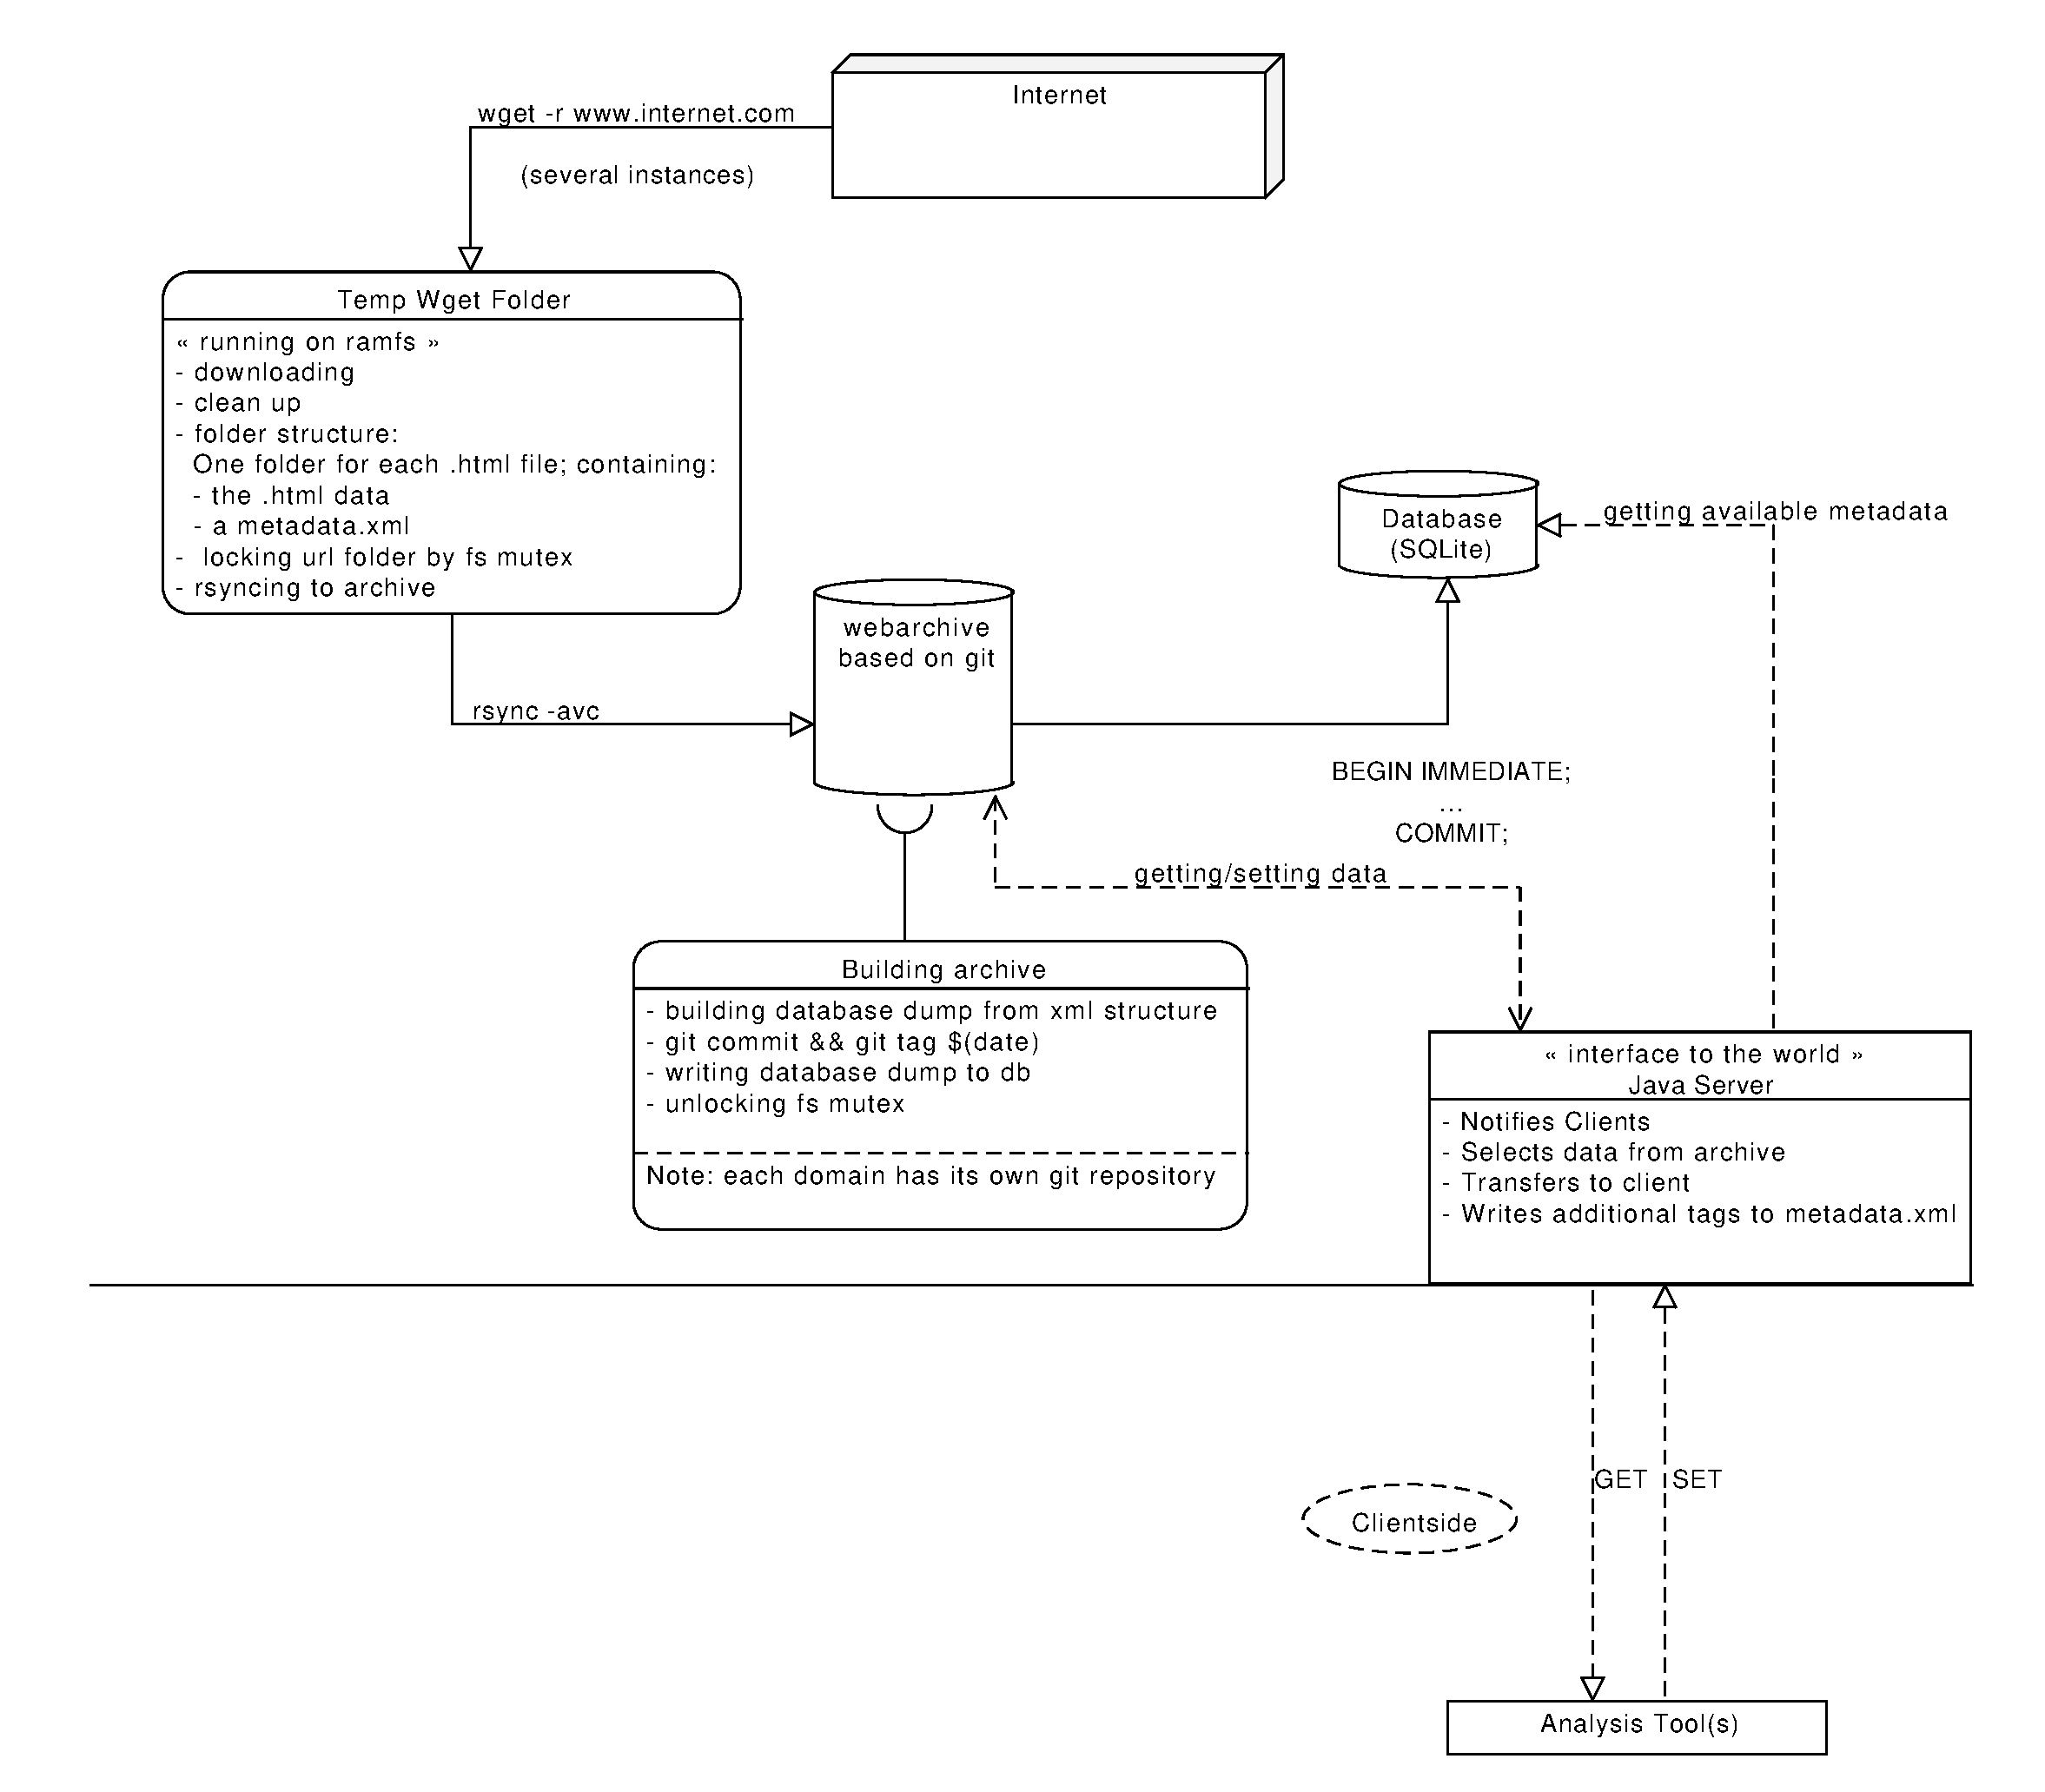
\includegraphics[width=\textwidth]{spezi/webarchiv_design.pdf}
	\caption{Diagramm: Grundlegendes Design}
\end{figure}
Die Steuerung erfolgt über ein Configfile (optional Kommandozeileninterface).
Es können folgende Parameter eingestellt werden:
\begin{itemize}
	\item Crawltiefe
	\item Zeitintervalle der Crawlvorgänge
	\item maximale Anzahl der gleichzeitig gestarteten Crawlerinstanzen
	\item Domains, also die Startpunkte für die Crawler, pro Domain wird dann ein Crawler gestartet,
		bis die Obergrenze erreicht wurde.
\end{itemize}

\chapter{Archiv}
Das Verzeichnis ist in einzelne Domainordner getrennt. Jeder Domainordner wird über ein Versionsverwaltung
(z.B. git) versioniert. Damit ist das Wiederherstellen älterer Versionen grundsätzlich möglich.
Beim Dateisystem wird von einem Linuxsystem ausgegangen.

\chapter{XML-Metadaten}
Die XML-Datei enthält grundsätzliche Metainformationen über eine archivierte HTML-Datei.
Die XML-Datei soll auch nachträglich über eine Programmierschnittstelle um weitere xml-tags erweiterbar sein.
Folgende Informationen stehen bereits fest: 
\begin{itemize}
	\item Git Commit Tag
	\item URL
	\item Dateipfad im Archiv
	\item Hashsumme über den Content
\end{itemize}

\chapter{Datenbank}
Die Datenbank dient zur Speicherung der grundlegenden Metadaten.
Diese soll während des Crawlvorgangs auf dem neuesten Stand gehalten werden.
Sollte die Datenbank beschädigt oder geändert werden, dann soll diese wieder aus den
XML-Metadaten rekonstruiert werden können.
 
\chapter{Crawlvorgang}
Für die Crawlerinstanzen wird ein externes Tool verwendet (z.B. wget).
Jede Instanz kopiert den Inhalt der Seite in je ein temporäres Verzeichnis.
Dabei sollen die HTML-Dateien je Domain in einen Ordner geschrieben werden.
Nach diesem Vorgang werden die tmp-Ordner bereinigt (z.B. leere Ordner entfernt)
und die HTML-Dateien in einen Ordner gleichen Namens kopiert.
Nun werden die Metadateien im XML-Format extrahiert und im o.g. Ordner gespeichert.
Zuletzt werden die so vorbereiteten tmp-Ordner in das vorhandene Archivverzeichnis
hineinsynchronisiert (z.B. mit rsync). Dabei wird jeder Domainordner über ein Dateimutex gelockt, um
gleichzeitiges Schreiben zu verhindern.
Zum Abschluss werden die Änderungen den Versionsverwaltungen der Domainordner mit einem Commit bestätigt.
Während oder nach dem Synchronisationsvorgang wird ein Datenbank-dump für die neuen oder geänderten Daten
erstellt. 

\chapter{Programmierschnittstelle - Java-Client}
Über diesen Client können vorbereitete Sql-Statements an einen Java-Server geschickt werden. Als return-Wert
wird eine Liste von Metadatenobjekten zurückgegeben.
Über diese Metadatenobjekte kann man sich nun über eine Anfrage die vorhandenen Archivordner aus dem Archiv herunterladen.
Auch eine Erweiterung der XML-Dateien um neue Tags bzw. die Abfrage von Tags soll über die 
Metadatenobjekte möglich sein.
Bei schreibendem Zugriff auf das Archiv muss immer auf das Setzen von Dateilocks geachtet werden.

% Diagramm

 

\end{document}



